%!TEX root = ../thesis.tex
This section will focus on describing and discussing a selection of concepts for ad hoc interfaces based the jamming technique.
As mentioned in the beginning of this chapter we were not successful at implementing a working jamming system where we could control air/liquid flow. \todo{make sure this is actually addressed. Suggestions: complexity, price of equipment: mechanics is one thing, the other is materials, i.e. ecoflex rubber etc.}
Therefore we concentrate on conceptual prototypes which we envisioned before taking the decision to move in other directions.

\subsection{Dynamic input controls} 

\todo{what's the problem with static dashboards}\\

Cell-based jamming, as mentioned in \ref{ch:jamming}, allows for deformations of individual cells.
This technique \hl{opens up} for a new and very dynamic approach to inputs, such as buttons, knobs, etc.
These input controls could emerge from the otherwise flat surface when needed, see figure~\ref{fig:ch:jamming:concepts:button}.
Other than being able to hide input controls when not needed this approach also opens up for a configurable interface adapted to a specific user's preference.
\citet{harrison2009providing} have previously made a contribution to physically changeable visual displays.
Their approach is not based on jamming but also on a pneumatic actuation which allow surface deformations of a latex surface.
This approach makes it possible to programmatically modify input control between three states: positive, neutral and negative, see figure~\ref{fig:ch:jamming:concepts:harrisonhudson}.
Though input controls are deformable and have tactile qualities, the displays are still in a very static configuration.
The positioning and shape of input controls are based on a backing layer with cut-out areas which cannot be changed.

\begin{figure}[h]
  \centering
      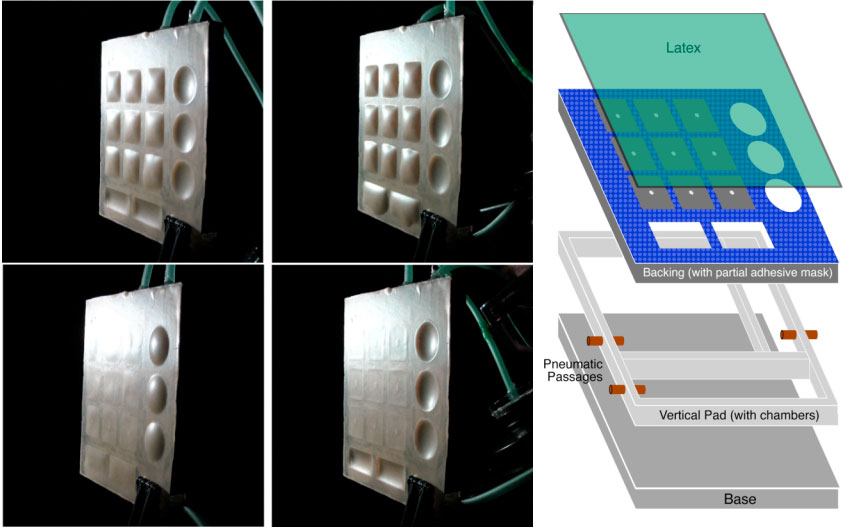
\includegraphics[width=.8\textwidth]{figures/jamming/concepts/harrisonhudson}
  \caption[A tactile display in various interfaces states. All buttons are statically positioned.]
  {A tactile display in various interfaces states. All buttons are statically positioned.}
  \label{fig:ch:jamming:concepts:harrisonhudson}
\end{figure}


\begin{verbatim}
kageform paper
\end{verbatim}

\begin{figure}[h]
  \centering
      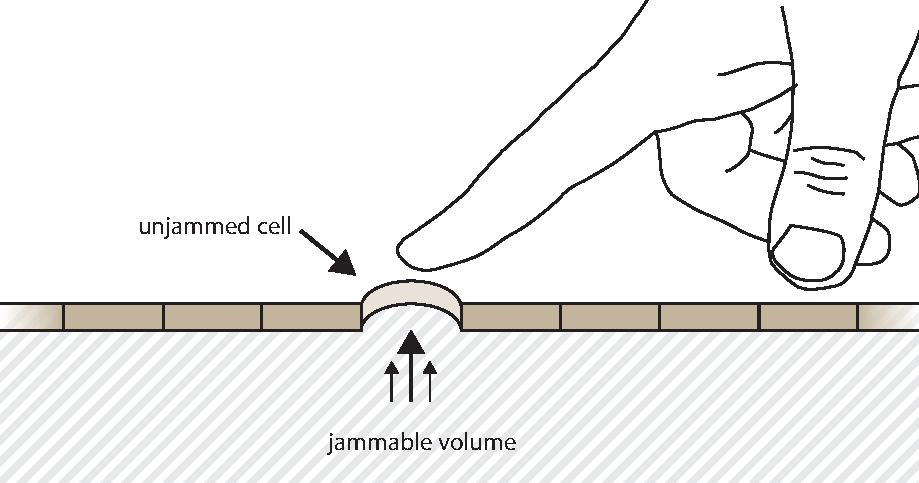
\includegraphics[width=3in]{figures/jamming/concepts/jamming_button}
  \caption[A cell-based jammable button.]
  {A cell-based jammable button.}
  \label{fig:ch:jamming:concepts:button}
\end{figure}

We conceptualize on household appliances such as radios, clock alarms, house alarms heating, ventilation and air conditioning (HVAC), \todo{etc}.
In general physical products with standard input controls such as buttons, knobs, switches and sliders.

with dynamic non-static interfaces.

\begin{verbatim}
1. dynamisk input kontrol
2. input + output kombination - ishii + rund robot (standard verbs)
	copy, paste, undo, delete form - digitale -> fysiske verden.
3. improviseret moebler (det fuldstaendig modelerbare hjem - tanken om at man kan tage selve strukturen af huset ned paa et niveau hvor man kan aendre i hoejere grad.)

\end{verbatim}
